% !TEX TS-program = pdflatex
% !TEX encoding = UTF-8 Unicode

% This is a simple template for a LaTeX document using the "article" class.
% See "book", "report", "letter" for other types of document.

\documentclass[11pt]{article} % use larger type; default would be 10pt

\usepackage[utf8]{inputenc} % set input encoding (not needed with XeLaTeX)

%%% Examples of Article customizations
% These packages are optional, depending whether you want the features they provide.
% See the LaTeX Companion or other references for full information.

%%% PAGE DIMENSIONS
\usepackage{geometry} % to change the page dimensions
\geometry{a4paper} % or letterpaper (US) or a5paper or....
% \geometry{margin=2in} % for example, change the margins to 2 inches all round
% \geometry{landscape} % set up the page for landscape
%   read geometry.pdf for detailed page layout information

\usepackage{graphicx} % support the \includegraphics command and options

% \usepackage[parfill]{parskip} % Activate to begin paragraphs with an empty line rather than an indent

%%% PACKAGES
\usepackage{booktabs} % for much better looking tables
\usepackage{array} % for better arrays (eg matrices) in maths
\usepackage{paralist} % very flexible & customisable lists (eg. enumerate/itemize, etc.)
\usepackage{verbatim} % adds environment for commenting out blocks of text & for better verbatim
\usepackage{subfig} % make it possible to include more than one captioned figure/table in a single float
% These packages are all incorporated in the memoir class to one degree or another...

%%% HEADERS & FOOTERS
\usepackage{fancyhdr} % This should be set AFTER setting up the page geometry
\pagestyle{fancy} % options: empty , plain , fancy
\renewcommand{\headrulewidth}{0pt} % customise the layout...
\lhead{}\chead{}\rhead{}
\lfoot{}\cfoot{\thepage}\rfoot{}

%%% SECTION TITLE APPEARANCE
\usepackage{sectsty}
\allsectionsfont{\sffamily\mdseries\upshape} % (See the fntguide.pdf for font help)
% (This matches ConTeXt defaults)

%%% ToC (table of contents) APPEARANCE
\usepackage[nottoc,notlof,notlot]{tocbibind} % Put the bibliography in the ToC
\usepackage[titles,subfigure]{tocloft} % Alter the style of the Table of Contents
\renewcommand{\cftsecfont}{\rmfamily\mdseries\upshape}
\renewcommand{\cftsecpagefont}{\rmfamily\mdseries\upshape} % No bold!

%%% END Article customizations

%%% The "real" document content comes below...

\title{Figures to insert in text}
\author{Author}
%\date{} % Activate to display a given date or no date (if empty),
         % otherwise the current date is printed

\begin{document}
\maketitle

\section{First section}

Your text goes here.

% FIGURES FIGURES FIGURES FIGURES FIGURES FIGURES FIGURES FIGURES FIGURES FIGURES FIGURES
\begin{figure}[h!]
  \centering
  \subfloat[$z \in \{.1, .2, .3, .4, .5, 1\}$]{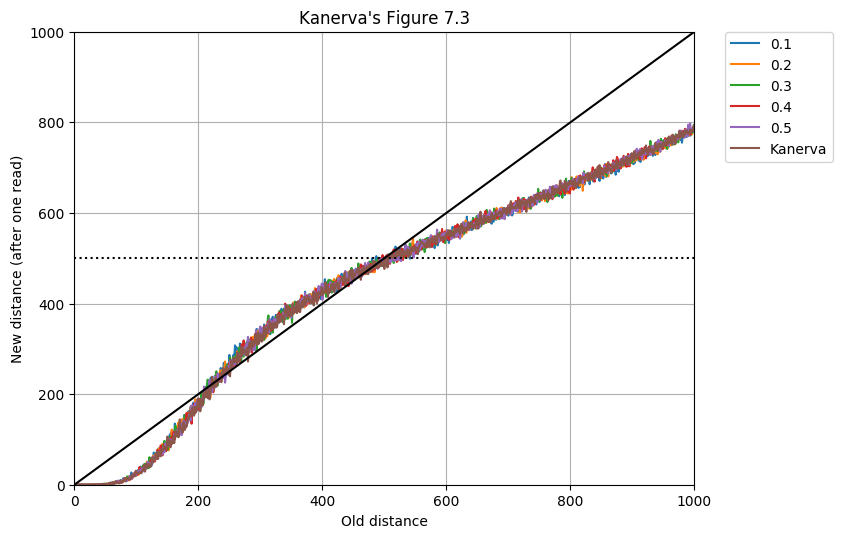
\includegraphics[width=2.9in]{./images02/new-images/iter_z_01-05.png}}
  \subfloat[$z \in \{1.5, 3, 4.5, 6\}$]{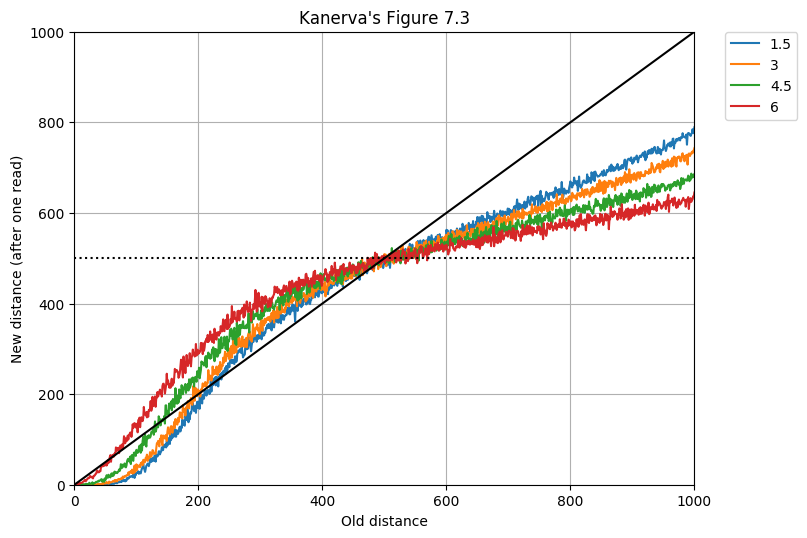
\includegraphics[width=2.9in]{./images02/new-images/z_15_3_45_6.png}}

  \subfloat[$z \in \{0, 1\}$]{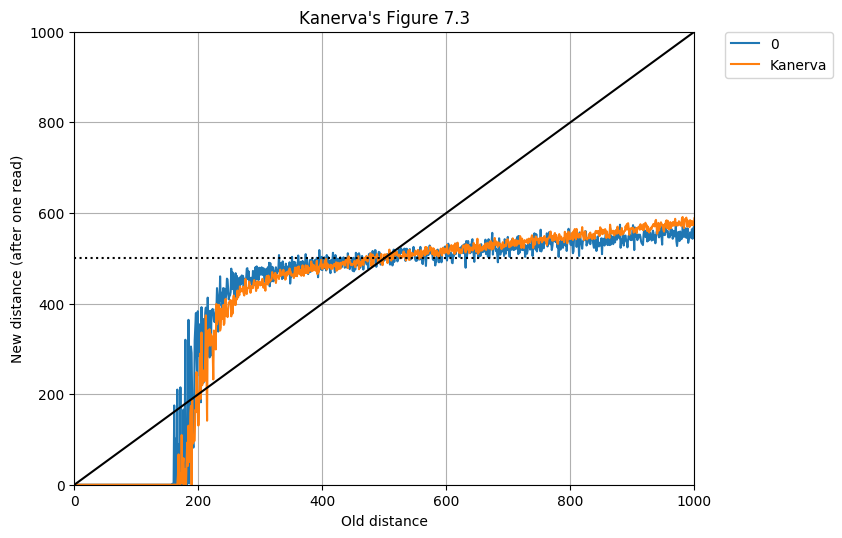
\includegraphics[width=2.9in]{./images02/new-images/z_0_1.png}}
  \subfloat[$z \in \{0, 0.5, 1, 1.5, 3, 4.5, 6\}$]{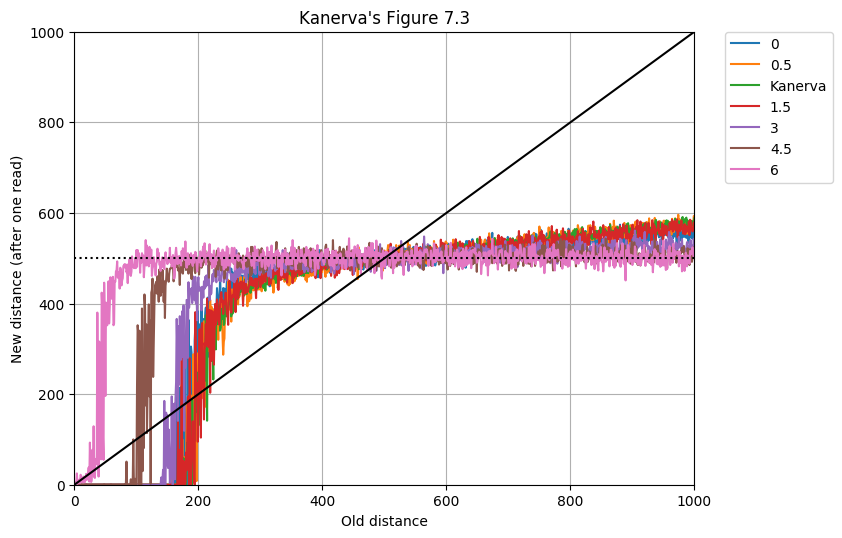
\includegraphics[width=2.9in]{./images02/new-images/iter_z_all_2.png}}

  \caption{Physicist Paulo Murillo observed that the models of Kanerva-read ($z=1$) and Chada-read ($z=0$) were simple variations of the exponent $z$, which suggests experimenting with different values. The results, however, have not yielded performance improvements.  Though for $z \leq 1$ results are comparable to $z=1$, for $z>1$, the system shows a clear deterioration, with a smaller distance to convergence and higher divergence at large-distance reads. (a) and (b) show the behavior of a single read; (c) and (d) present the effects of 6 iterative reads. As stated previously, we can see a deterioration of convergence, with lower critical distance as $z>1$.  Another observation can be made here, concerning the discrepancy of Kanerva's Fig 7.3 and our data.  It seems that Kanerva did not consider that a single read would only `clean' a small number of dimensions \emph{after the critical distance}. What we observe clearly is that with a single read, as the distance grows, the system only `cleans' towards the orthoghonal distance 500 after a number of iterative readings.}
  \label{fig:murillo-generalization-experiments}
\end{figure}

% FIGURES ITER FIGURES ITER FIGURES FIGURES FIGURES FIGURES FIGURES FIGURES FIGURES FIGURES FIGURES

\section{Critical Distance Analysis: a brief review}

\begin{figure}[h!]
\centering

\subfloat[Kanerva's original model]{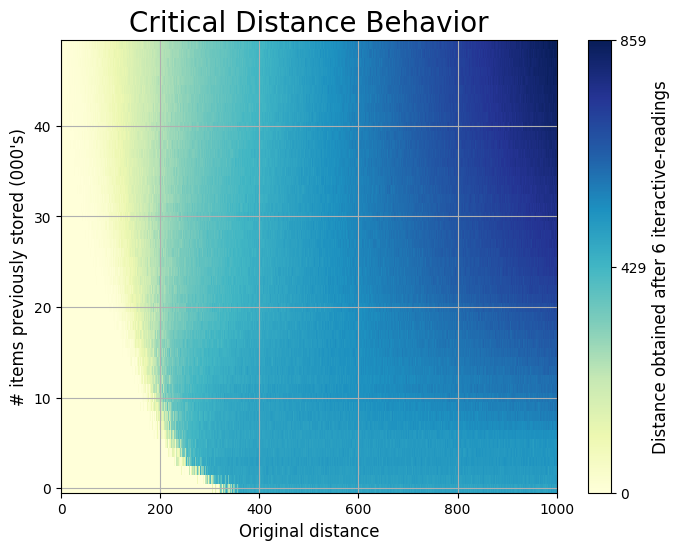
\includegraphics[width=3.1in]{./images02/new-images/kanerva-read.png}}

\subfloat[Chada's read]{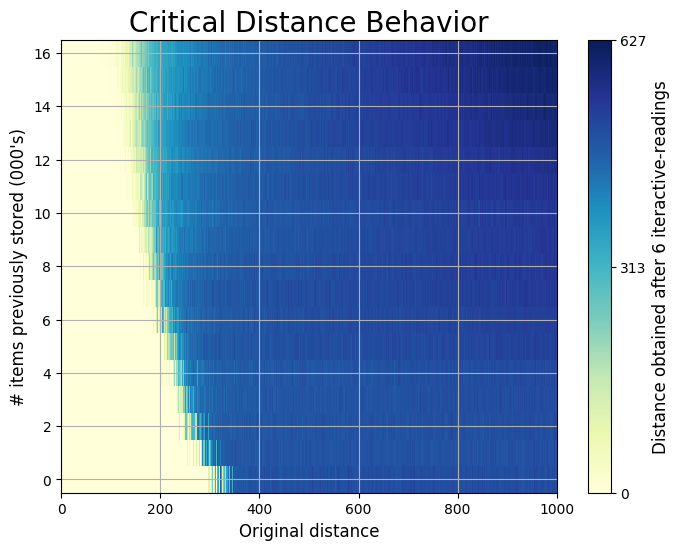
\includegraphics[width=3.1in]{./images02/new-images/chada-read_z_0.png}}
\caption{How far, in hamming distance, is a read item from the original stored item? Kanerva demonstrated that, after a small number of iterative readings (6 here), a critical distance behavior emerges. Items read at close distance converge rapidly; whereas farther items do not converge. Most striking is the point in which the system displays the tip-of-tongue behavior. Described by psychological moments when some features of the item are prominent in one's thoughts, yet the item still cannot be recalled (but an additional cue makes convergence `immediate'). Mathemathically, this is the precise distance in which, despite having a relatively high number of cues (correct bits) about the desired item, the time to convergence is infinite.   Heatmap colors display the hamming distance the associative memory is able to cleanly converge to---or not.   In the $x$-axis, the distance from the desired item is displayed. In the $y$-axis, we display the read operation's behavior as the number of items registered in the memory grows.  These graphs are computing intensive, yet they can be easily tested by readers in our provided jupyter notebooks. Note the different scales.}
\label{fig:crit-dist-10k-writes}

\end{figure}

Figure \ref{fig:Crit-Dist-Comparison} compares the critical distance behavior under different scenarios.


\section{Speculations on the use of Information Theory}

\begin{figure}
  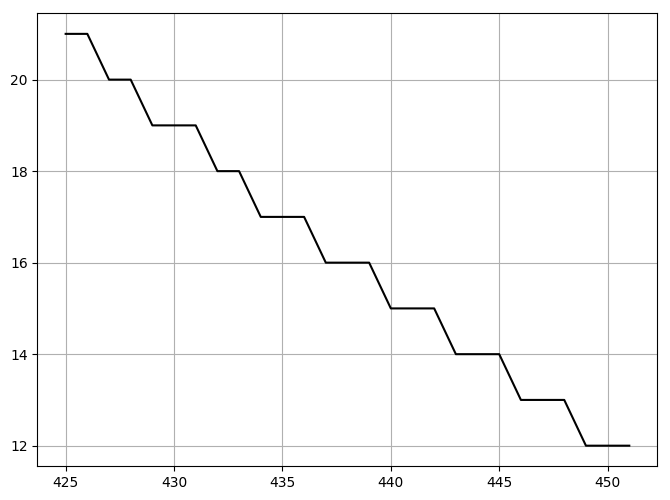
\includegraphics[width=\linewidth]{./images02/new-images/information_decay.png}
  \caption{information decay 4.png}
  \label{fig:boat10}
\end{figure}


\subsection{A subsection}

More text.

\end{document}
